\item \subquestionpoints{4} {\bf Coding question: other feature maps}

You may have observed that it requires a relatively high degree $k$ to fit the given training data, and this is because the dataset cannot be explained (i.e., approximated) very well by low-degree polynomials. By visualizing the data, you may have realized that $y$ can be approximated well by a sine wave. In fact, we generated the data by sampling from $y = \sin(x) + \xi$, where $\xi$ is noise with Gaussian distribution. Please update the feature map $\phi$ to include a sine transformation as follows:

\begin{align}
\phi(x) = \left[\begin{array}{c} 1\\ x \\ x^2\\ \vdots \\x^k \\ \sin(x) \end{array}\right]\in \mathbb{R}^{k+2} \label{eqn:feature-sine}
\end{align}

With the updated feature map, train different models for values of $k=0,1,2,3,5,10,20$, and plot the resulting hypothesis curves over the data as before.

Submit the plot as a solution to this sub-problem. Compare the fitted models with the previous sub-question, and briefly comment about noticable differences in the fit with this feature map.\\

Your plot should look similar to the following:
\begin{figure}[H]
  \centering
  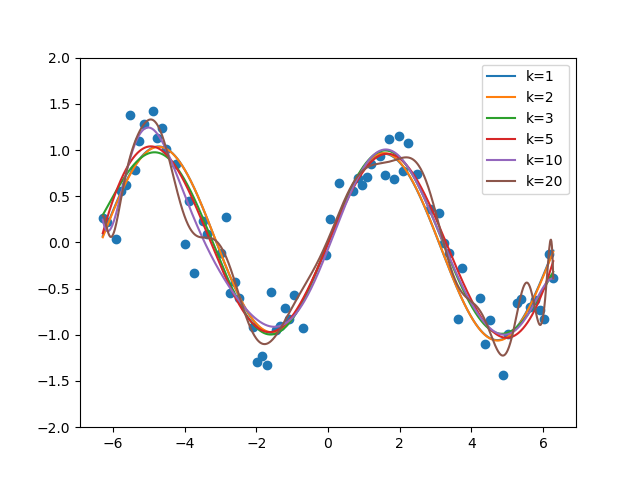
\includegraphics[width=0.65\linewidth]{featuremaps/src/large-sine.png}
  \centering
\caption{Polynomial regression with other features with kernel sizes 1,2,3,5,10 and 20}
\end{figure}

Provide your comparison of the fitted models here:\\[50pt]